\documentclass[11pt]{article}

\usepackage[a4paper,margin=1in]{geometry}
\usepackage[T1]{fontenc}
\usepackage[utf8]{inputenc}
\usepackage{lmodern}
\usepackage{setspace}
\usepackage{amsmath,amssymb}
\usepackage{booktabs}
\usepackage{graphicx}
\usepackage{float}
\usepackage{caption}
\usepackage{subcaption}
\usepackage{hyperref}
\usepackage[nameinlink]{cleveref}
\usepackage[authoryear]{natbib}

\newcommand{\parencite}[1]{\citep{#1}}
\newcommand{\textcite}[1]{\citet{#1}}

\title{Robust Benchmark-Relative Tests of Weak-Form Efficiency\\
in Latin American Equity ETFs}
\author{Leonardo H. Talero-Sarmiento}
\date{\today}

\begin{document}
\onehalfspacing
\maketitle

\begin{abstract}
This paper evaluates weak-form efficiency in four Latin American equity ETFs (EWZ, EWW, ECH, GXG) using benchmark-relative out-of-sample forecasting tests. The estimand is forecast-loss difference versus a random-walk baseline under a common lagged information set. We implement expanding-window evaluation with horizon gap controls, leakage assertions, and multiple loss metrics (RMSE, MAE, directional accuracy) across six $(L,H)$ configurations. Benchmarks include random walk, historical mean, linear autoregressive, ridge, MLP, and random-forest models, with conditional diffusion evaluated under the same target definition and window protocol.

Random walk remains the lowest-RMSE model in all tested configurations. At short horizon ($H=1$), some simple alternatives are close to random walk but gains are weak or unstable across settings. Diffusion underperforms benchmark models materially and is significantly worse than random walk in all Diebold-Mariano comparisons in this implementation. Diffusion seed and feature ablations indicate substantial sensitivity, and XAI reliance patterns are not stable enough for strong structural interpretation. Findings are therefore interpreted as disciplined evidence of limited extractable short-horizon predictability, not as proof of exploitable inefficiency.
\end{abstract}

\section{Introduction}

Weak-form market efficiency remains a core benchmark in empirical finance. In emerging markets, however, integration frictions, episodic illiquidity, and structural regime changes motivate repeated reassessment of short-horizon predictability \parencite{fama1970,fama1991,harvey1995,bekaertharvey1995}.

This study asks one focused question:
\begin{quote}
Do diffusion-based forecasts deliver robust out-of-sample loss reductions relative to strong benchmark models for Latin American ETF cumulative returns?
\end{quote}

The empirical contribution is a benchmark-disciplined comparison across EWZ, EWW, ECH, and GXG over six $(L,H)$ configurations with expanding-window evaluation and Diebold-Mariano inference against random walk. The methodological contribution is a leakage-audited, horizon-consistent workflow that combines classical baselines, nonlinear baselines, conditional diffusion, and seed/feature sensitivity analysis under a common target definition. The interpretability contribution is a stability-oriented XAI layer that treats feature reliance as predictive model dependence, not causal mechanism.

Inference is intentionally conservative. The design supports statements about forecast association and incremental predictive content; it does not identify causal effects, structural transmission parameters, or implementable profitability after transaction costs.

\section{Literature Positioning and Gap}

Weak-form efficiency and return-predictability studies show that apparent forecast gains are often unstable once out-of-sample discipline is imposed \parencite{lomackinlay1988,welchgoyal2008,campbellthompson2008,rapach2010}. In emerging markets, integration and information-friction mechanisms motivate context-specific reassessment rather than universal claims \parencite{harvey1995,bekaertharvey1995}. For Latin America, much of the evidence remains concentrated in variance-ratio, adaptive-market, or related dependence-testing traditions \parencite{urrutia1995,sanchezgranero2020,lo2004,cruzhernandez2024}, while large-scale machine-learning evidence is mostly developed-market focused \parencite{gu2020}. Diffusion methodology is technically mature in machine learning \parencite{ho2020,song2021}, and finance applications are emerging \parencite{cho2026}, but benchmark-disciplined weak-form tests in this LatAm ETF setting remain limited.

The gap is therefore not the absence of EMH tests, but the absence of a coherent benchmark-first forecast-comparison design that separates predictive association from structural inefficiency claims. This paper addresses that gap by combining leakage-audited target construction, expanding-window evaluation, strong baseline comparators, formal loss-differential inference, and explicit interpretation boundaries for EMH.

\section{Data and Variable Construction}

\subsection{Data Source and Scope}
Raw adjusted-close prices and volumes are downloaded from Yahoo Finance through \texttt{yfinance}. The empirical assets are EWZ (Brazil), EWW (Mexico), ECH (Chile), and GXG (Colombia). Frequency is daily.

\begin{table}[!htbp]
\centering
\caption{Data overview.}
\label{tab:data-overview}
\begin{tabular}{lr}
\toprule
Item & Value \\
\midrule
Assets & 4 \\
Observations (daily) & 2264 \\
Start date & 2015-01-02 \\
End date & 2023-12-29 \\
Average active mask & 1.000 \\
\bottomrule
\end{tabular}
\caption*{\footnotesize Raw data source: Yahoo Finance via yfinance; assets: EWZ, EWW, ECH, GXG.}
\end{table}


\Cref{tab:data-overview} reports the effective sample (2015-01-02 to 2023-12-29, 2,264 daily observations). The preprocessing pipeline is deterministic: prices are forward-filled, returns are computed from adjacent adjusted closes, and a tradability mask suppresses inactive observations (missing price or non-positive volume).

\subsection{Variable Construction}
For asset $i$ at date $t$, let $P_{i,t}$ denote adjusted close and $V_{i,t}$ traded volume. The tradability mask is
\begin{equation}
m_{i,t} = \mathbb{1}\!\left(P_{i,t}\text{ observed and }V_{i,t}>0\right).
\label{eq:mask}
\end{equation}

The daily log return is
\begin{equation}
r_{i,t} = \log\!\left(\frac{P_{i,t}}{P_{i,t-1}}\right)m_{i,t}.
\label{eq:return}
\end{equation}

Following \textcite{amihud2002}, the illiquidity proxy is
\begin{equation}
\text{illiq}_{i,t} = \frac{|r_{i,t}|}{P_{i,t}V_{i,t}+\varepsilon}, \quad \varepsilon=10^{-8},
\label{eq:amihud}
\end{equation}
and standardized with a 60-day rolling window:
\begin{equation}
z^{\text{illiq}}_{i,t} = \frac{\text{illiq}_{i,t}-\mu_{i,t}^{(60)}}{\sigma_{i,t}^{(60)}+\varepsilon}.
\label{eq:amihud-z}
\end{equation}
with \(\mu_{i,t}^{(60)}\) and \(\sigma_{i,t}^{(60)}\) denoting rolling mean and standard deviation. Values undefined in early windows are set to zero in the processed feature matrix.

The model context at forecast origin $t$ is
\begin{equation}
\mathcal{X}_{t}=\left\{r_{i,\tau},m_{i,\tau},z^{\text{illiq}}_{i,\tau}\right\}_{i=1,\ldots,N;\,\tau=t-L,\ldots,t-1}.
\label{eq:context}
\end{equation}

The $H$-day forecast target is cumulative return
\begin{equation}
y^{(H)}_{i,t} = \sum_{j=0}^{H-1} r_{i,t+j}.
\label{eq:target}
\end{equation}
which matches the implementation in the dataset loader used by all competing models.

\section{Econometric Strategy and Identification}

\subsection{Object of Inference}
The core estimand is benchmark-relative out-of-sample loss improvement versus random walk. For candidate model \(m\),
\begin{equation}
\Delta \mathcal{L}_{m} = \mathbb{E}\!\left[\ell\!\left(e_t^{\mathrm{rw}}\right)-\ell\!\left(e_t^{m}\right)\right],
\end{equation}
where \(\ell(\cdot)\) is forecast loss and \(e_t^{m}=y_t-\hat{y}_t^{m}\). Positive values indicate lower loss than random walk. The design identifies predictive association only.

\subsection{Temporal Integrity and Leakage Controls}
Leakage safeguards are imposed at preprocessing, sample construction, and validation stages.
\begin{enumerate}
  \item Processed feature indices are required to be time-sorted, unique, and aligned across returns, mask, and illiquidity inputs.
  \item The illiquidity standardization uses strictly lagged rolling moments in code, so statistics at \(t\) are computed from data up to \(t-1\).
  \item For each origin \(i\), context uses \([i-L,\ldots,i-1]\) and target uses \([i,\ldots,i+H-1]\).
  \item Expanding-window evaluation inserts a horizon gap \(H-1\) between training and validation origins, and assertions fail if target windows overlap.
\end{enumerate}

\subsection{Validation Design}
Instead of a single split, each \((L,H)\) configuration is evaluated on multiple expanding windows. Let \(w\in\{1,\ldots,W\}\) index windows. For each \(w\), models are fitted on a chronological training block and evaluated on a later validation block. Per-window losses are stored and aggregated, and \(W\) is reported with each summary metric.

\subsection{Competing Forecast Models}
All models forecast the same cumulative-return target from comparable lagged information sets:
\begin{enumerate}
  \item \textbf{Random walk} (\(\hat{y}_{i,t}^{(H)}=0\)).
  \item \textbf{Historical mean} (mean lagged return in lookback window).
  \item \textbf{Linear autoregressive baseline} (asset-wise linear AR on lagged returns).
  \item \textbf{Ridge regression} on flattened context with time-aware inner validation for \(\alpha\).
  \item \textbf{Shallow MLP baseline} with train-only scaling and early stopping.
  \item \textbf{Random-forest baseline} (parsimonious tree depth and leaf-size controls).
  \item \textbf{Conditional diffusion model}.
\end{enumerate}

For diffusion with schedule \(\{\beta_s\}_{s=1}^{S}\), define \(\alpha_s=1-\beta_s\), \(\bar{\alpha}_s=\prod_{u=1}^{s}\alpha_u\), and
\begin{equation}
y_s = \sqrt{\bar{\alpha}_s}\,y_0 + \sqrt{1-\bar{\alpha}_s}\,\epsilon, \quad \epsilon\sim\mathcal{N}(0,I).
\end{equation}
The denoiser \(\epsilon_{\theta}\) is trained by
\begin{equation}
\min_{\theta}\;\mathbb{E}_{y_0,\epsilon,s}\!\left[\left\|\epsilon-\epsilon_{\theta}(y_s,s,\mathcal{X}_t)\right\|_2^2\right].
\label{eq:ddpm-loss}
\end{equation}
Training uses fixed conservative hyperparameters, seed control, and an inner time-ordered validation split with early stopping.

\subsection{Loss Metrics and Comparative Inference}
Point-forecast losses include RMSE and MAE:
\begin{equation}
\text{RMSE}=
\sqrt{
\frac{1}{TN}
\sum_{t=1}^{T}\sum_{i=1}^{N}
\left(y_{i,t}^{(H)}-\hat{y}_{i,t}^{(H)}\right)^2
}, \quad
\text{MAE}=
\frac{1}{TN}\sum_{t=1}^{T}\sum_{i=1}^{N}
\left|y_{i,t}^{(H)}-\hat{y}_{i,t}^{(H)}\right|.
\end{equation}
Directional accuracy is reported as a complementary diagnostic.

Forecast comparison uses Diebold--Mariano tests \parencite{dieboldmariano1995} with
\begin{equation}
d_t=\ell(e_t^{\mathrm{rw}})-\ell(e_t^{m}), \qquad
\text{DM}=\frac{\bar{d}}{\sqrt{\widehat{v}_d/T}}.
\label{eq:dm}
\end{equation}
Under this sign convention, negative DM indicates higher loss for the candidate model than random walk.

\subsection{Robustness and Sensitivity Design}
Robustness dimensions include horizon (\(H\)), lookback (\(L\)), window-to-window stability, diffusion seed sensitivity, and feature-set ablations (\texttt{full}, \texttt{no\_illiquidity}, \texttt{returns\_only}). XAI analysis is framed as model reliance and explanation stability, not causality.

\section{Empirical Results}

\subsection{Descriptive Properties}
\begin{table}[!htbp]
\centering
\caption{Summary statistics of daily log returns.}
\label{tab:summary-statistics}
\begin{tabular}{lrrrrr}
\toprule
ETF & Mean & Std. Dev. & Skewness & Kurtosis & ACF(1) \\
\midrule
ECH & -0.00002 & 0.01733 & -0.624 & 10.600 & -0.012 \\
EWW & 0.00016 & 0.01597 & -1.068 & 9.448 & -0.010 \\
EWZ & 0.00018 & 0.02365 & -1.137 & 13.272 & -0.133 \\
GXG & -0.00020 & 0.01725 & -1.214 & 16.423 & 0.146 \\
\bottomrule
\end{tabular}
\end{table}

\begin{table}[!htbp]
\centering
\caption{Stationarity and serial dependence diagnostics.}
\label{tab:diagnostics}
\begin{tabular}{lrrrr}
\toprule
ETF & ADF p (price) & ADF p (return) & LB p (return) & LB p (return$^2$) \\
\midrule
ECH & 0.348 & 0.000 & 0.000 & 0.000 \\
EWW & 0.805 & 0.000 & 0.000 & 0.000 \\
EWZ & 0.094 & 0.000 & 0.000 & 0.000 \\
GXG & 0.050 & 0.000 & 0.000 & 0.000 \\
\bottomrule
\end{tabular}
\caption*{\footnotesize ADF is Augmented Dickey-Fuller test; LB is Ljung-Box at lag 10.}
\end{table}

\begin{table}[!htbp]
\centering
\caption{Pairwise correlation matrix of daily log returns.}
\label{tab:return-correlations}
\begin{tabular}{lrrrr}
\toprule
ETF & ECH & EWW & EWZ & GXG \\
\midrule
ECH & 1.000 & 0.586 & 0.568 & 0.581 \\
EWW & 0.586 & 1.000 & 0.662 & 0.611 \\
EWZ & 0.568 & 0.662 & 1.000 & 0.578 \\
GXG & 0.581 & 0.611 & 0.578 & 1.000 \\
\bottomrule
\end{tabular}
\end{table}


\Cref{tab:summary-statistics} shows near-zero unconditional mean returns with heavy tails. \Cref{tab:diagnostics} confirms stationary returns, mostly non-stationary price levels, and strong serial dependence in squared returns. \Cref{tab:return-correlations} indicates moderate cross-market comovement (off-diagonal correlations approximately 0.57--0.66), consistent with regional integration without near-collinearity.

\subsection{Baseline Benchmark Performance}
\begin{table}[!htbp]
\centering
\caption{Out-of-sample RMSE by lookback window and forecast horizon.}
\label{tab:rmse-by-config}
\begin{tabular}{lrrrrrrrr}
\toprule
L & H & AR Linear & Diffusion & Historical Mean & MLP & Random Forest & Random Walk & Ridge \\
\midrule
10 & 1 & 0.02016 & 0.02036 & 0.02093 & 0.11455 & 0.02012 & 0.02003 & 0.02045 \\
10 & 5 & 0.04630 & 0.04657 & 0.04629 & 0.11620 & 0.04641 & 0.04623 & 0.04658 \\
21 & 1 & 0.02020 & 0.02060 & 0.02055 & 0.18238 & 0.02018 & 0.02006 & 0.02058 \\
21 & 5 & 0.04633 & 0.04675 & 0.04650 & 0.19631 & 0.04660 & 0.04626 & 0.04740 \\
42 & 1 & 0.02027 & 0.02051 & 0.02035 & 0.30816 & 0.02021 & 0.02013 & 0.02096 \\
42 & 5 & 0.04653 & 0.04742 & 0.04652 & 0.29810 & 0.04695 & 0.04646 & 0.04891 \\
\bottomrule
\end{tabular}
\caption*{\footnotesize Lower values indicate better forecast accuracy.}
\end{table}

\begin{table}[!htbp]
\centering
\caption{Average losses and directional accuracy across expanding windows.}
\label{tab:model-performance-summary}
\begin{tabular}{lrrrrrr}
\toprule
L & H & Model & RMSE & MAE & Dir. Acc. & Windows \\
\midrule
10 & 1 & Random Walk & 0.02003 & 0.01436 & 0.007 & 5 \\
10 & 1 & Random Forest & 0.02011 & 0.01436 & 0.513 & 5 \\
10 & 1 & AR Linear & 0.02016 & 0.01448 & 0.511 & 5 \\
10 & 1 & Ridge & 0.02026 & 0.01459 & 0.499 & 5 \\
10 & 1 & Historical Mean & 0.02093 & 0.01518 & 0.503 & 5 \\
10 & 1 & MLP & 0.09460 & 0.06558 & 0.489 & 5 \\
10 & 1 & Diffusion & 0.48328 & 0.38319 & 0.501 & 5 \\
10 & 5 & Random Walk & 0.04623 & 0.03437 & 0.000 & 5 \\
10 & 5 & Historical Mean & 0.04629 & 0.03444 & 0.505 & 5 \\
10 & 5 & AR Linear & 0.04630 & 0.03441 & 0.506 & 5 \\
10 & 5 & Random Forest & 0.04657 & 0.03453 & 0.509 & 5 \\
10 & 5 & Ridge & 0.04659 & 0.03463 & 0.517 & 5 \\
10 & 5 & MLP & 0.11469 & 0.08301 & 0.502 & 5 \\
10 & 5 & Diffusion & 0.64470 & 0.51013 & 0.505 & 5 \\
21 & 1 & Random Walk & 0.02006 & 0.01440 & 0.007 & 5 \\
21 & 1 & Random Forest & 0.02019 & 0.01441 & 0.512 & 5 \\
21 & 1 & AR Linear & 0.02020 & 0.01452 & 0.511 & 5 \\
21 & 1 & Ridge & 0.02051 & 0.01480 & 0.492 & 5 \\
21 & 1 & Historical Mean & 0.02055 & 0.01484 & 0.508 & 5 \\
21 & 1 & MLP & 0.16236 & 0.11591 & 0.488 & 5 \\
21 & 1 & Diffusion & 0.48483 & 0.38419 & 0.491 & 5 \\
21 & 5 & Random Walk & 0.04626 & 0.03446 & 0.000 & 5 \\
21 & 5 & AR Linear & 0.04633 & 0.03451 & 0.508 & 5 \\
21 & 5 & Historical Mean & 0.04650 & 0.03460 & 0.511 & 5 \\
21 & 5 & Random Forest & 0.04664 & 0.03476 & 0.476 & 5 \\
21 & 5 & Ridge & 0.04737 & 0.03531 & 0.498 & 5 \\
21 & 5 & MLP & 0.20417 & 0.14775 & 0.498 & 5 \\
21 & 5 & Diffusion & 0.47032 & 0.37295 & 0.504 & 5 \\
42 & 1 & Random Walk & 0.02013 & 0.01446 & 0.007 & 5 \\
42 & 1 & Random Forest & 0.02023 & 0.01449 & 0.498 & 5 \\
42 & 1 & AR Linear & 0.02027 & 0.01459 & 0.509 & 5 \\
42 & 1 & Historical Mean & 0.02035 & 0.01466 & 0.503 & 5 \\
42 & 1 & Ridge & 0.02090 & 0.01513 & 0.505 & 5 \\
42 & 1 & MLP & 0.35766 & 0.26714 & 0.505 & 5 \\
42 & 1 & Diffusion & 0.55543 & 0.44136 & 0.493 & 5 \\
42 & 5 & Random Walk & 0.04646 & 0.03465 & 0.000 & 5 \\
42 & 5 & Historical Mean & 0.04652 & 0.03468 & 0.503 & 5 \\
42 & 5 & AR Linear & 0.04653 & 0.03469 & 0.507 & 5 \\
42 & 5 & Random Forest & 0.04689 & 0.03509 & 0.479 & 5 \\
42 & 5 & Ridge & 0.04872 & 0.03652 & 0.492 & 5 \\
42 & 5 & MLP & 0.34519 & 0.25755 & 0.498 & 5 \\
42 & 5 & Diffusion & 0.55365 & 0.43909 & 0.499 & 5 \\
\bottomrule
\end{tabular}
\end{table}


\begin{figure}[!htbp]
  \centering
  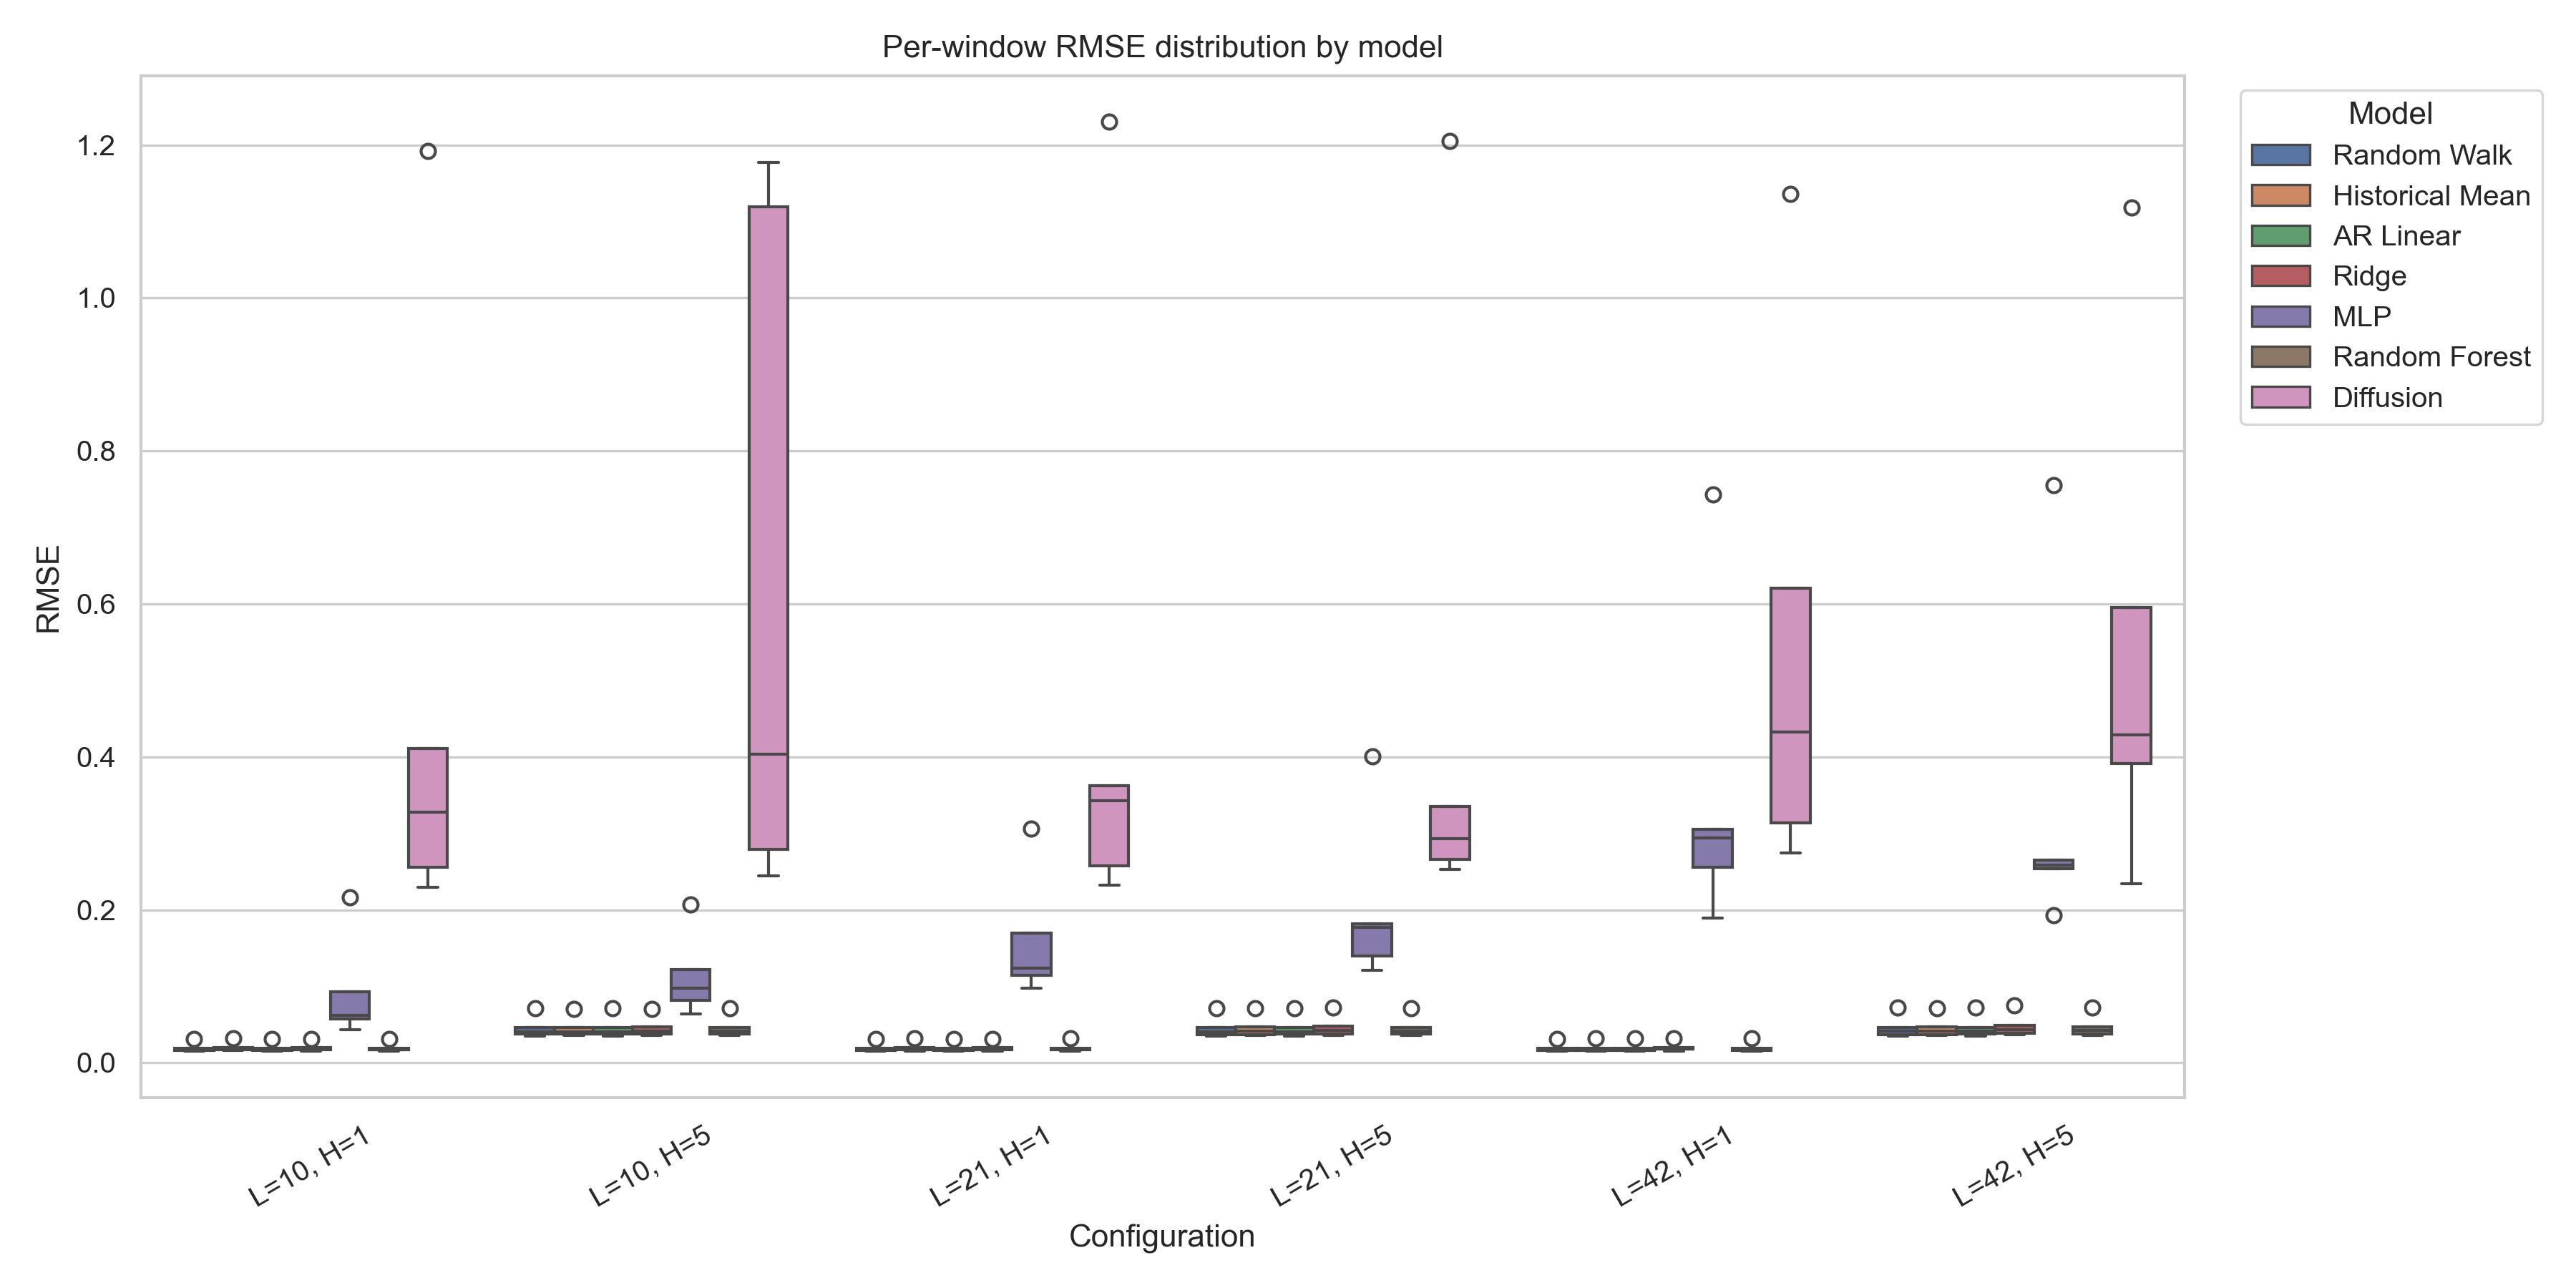
\includegraphics[width=0.96\linewidth]{../figures/generated/fig_rmse_by_model.png}
  \caption{Per-window RMSE distribution by model and configuration.}
  \label{fig:rmse}
\end{figure}

Random walk is the lowest-RMSE benchmark in all six \((L,H)\) configurations (\Cref{tab:rmse-by-config,tab:model-performance-summary,fig:rmse}). At \(H=1\), random-forest and linear-AR baselines are close to random walk in level terms but do not dominate consistently across lookback settings. At \(H=5\), historical mean and AR-linear models are again close to random walk, while more flexible ML models (MLP) degrade materially.

\subsection{Diffusion Model Performance}
Diffusion forecasts are worse than benchmark models in most configurations, but the absolute scale is close to the random-walk baseline: approximately 0.0201--0.0203 for \(H=1\) and 0.0464--0.0470 for \(H=5\) (\Cref{tab:rmse-by-config}).

\subsection{Formal Comparative Inference}
\begin{table}[!htbp]
\centering
\caption{Diebold-Mariano comparison versus random walk.}
\label{tab:dm-summary}
\begin{tabular}{lrr}
\toprule
Model & Mean DM statistic & Significant at 5\% \\
\midrule
AR Linear & -1.297 & 2 / 6 \\
Diffusion & -21.694 & 6 / 6 \\
Historical Mean & -1.594 & 3 / 6 \\
MLP & -11.505 & 6 / 6 \\
Random Forest & -2.002 & 3 / 6 \\
Ridge & -4.704 & 5 / 6 \\
\bottomrule
\end{tabular}
\caption*{\footnotesize Negative DM means the candidate model has higher loss than random walk.}
\end{table}


\begin{figure}[!htbp]
  \centering
  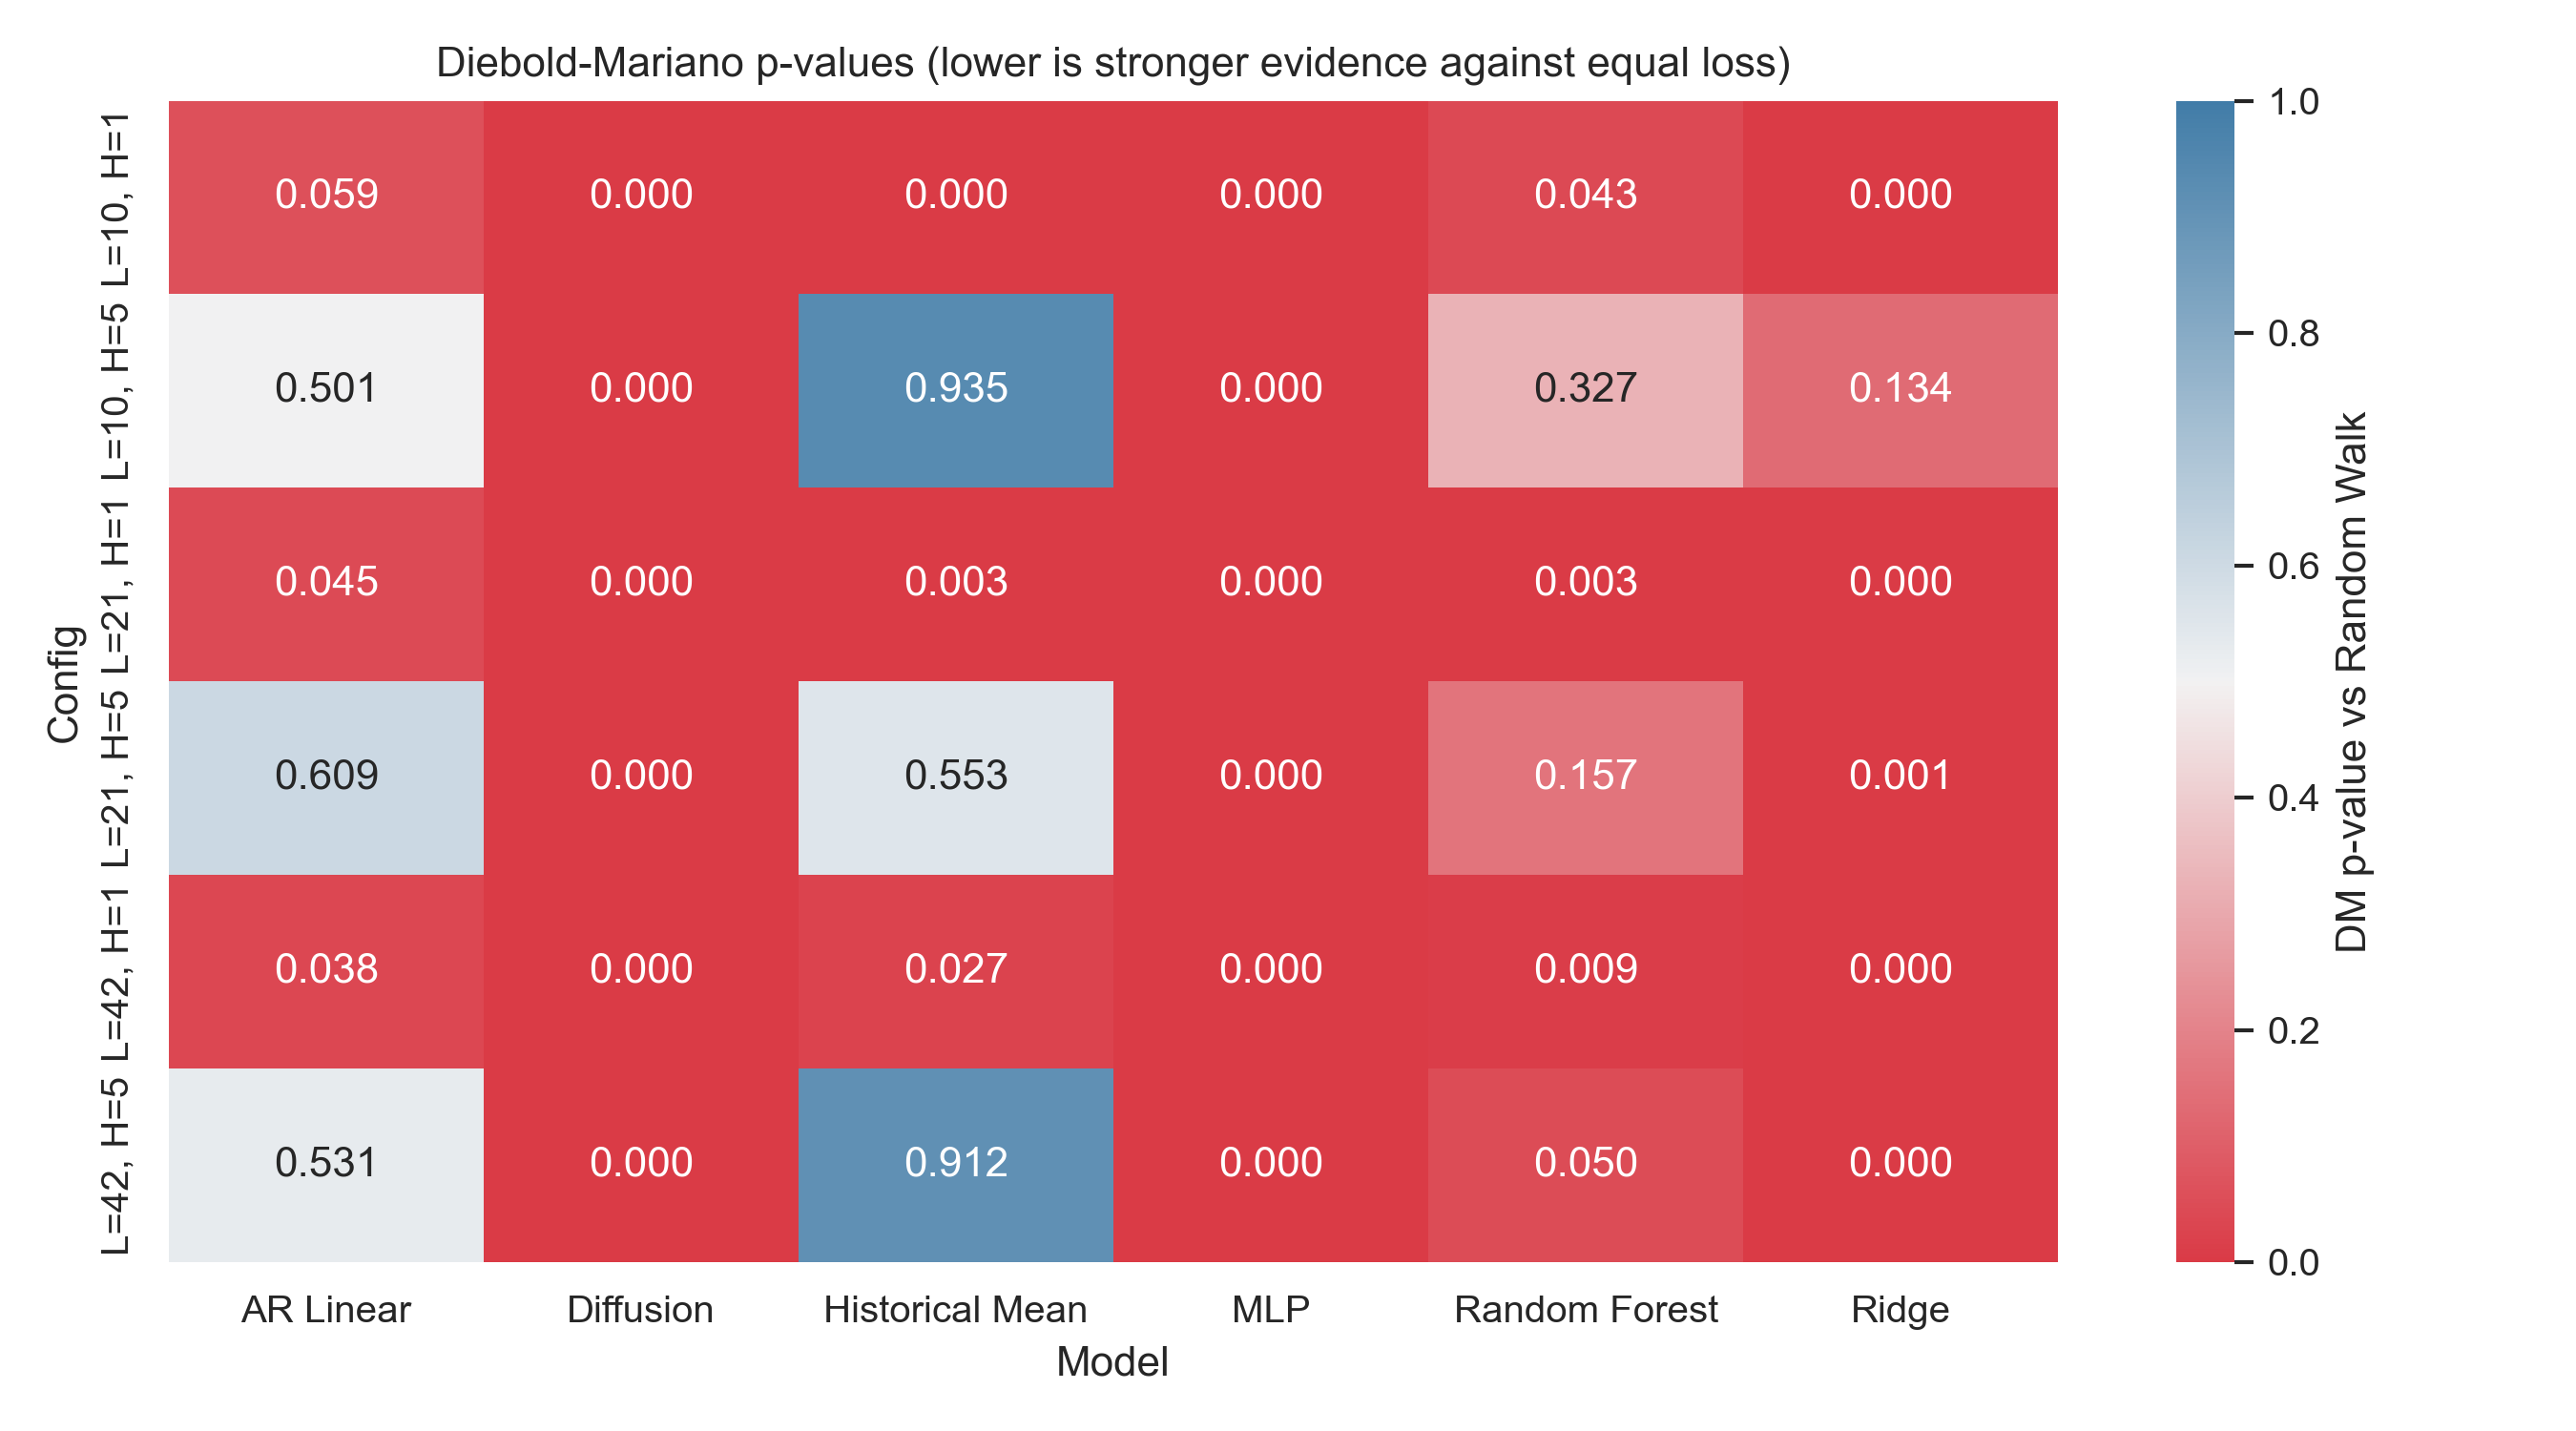
\includegraphics[width=0.86\linewidth]{../figures/generated/fig_dm_pvalue_heatmap.png}
  \caption{Diebold--Mariano p-values versus random walk.}
  \label{fig:dm-pvalue}
\end{figure}

\Cref{tab:dm-summary,fig:dm-pvalue} confirms that diffusion is significantly worse than random walk in four of six configurations under DM tests. At \(H=5\), diffusion is not significantly different from random walk for selected lookback settings, while ridge and MLP are typically inferior.

\subsection{XAI Findings}
\begin{figure}[!htbp]
  \centering
  \begin{subfigure}{0.49\linewidth}
    \centering
    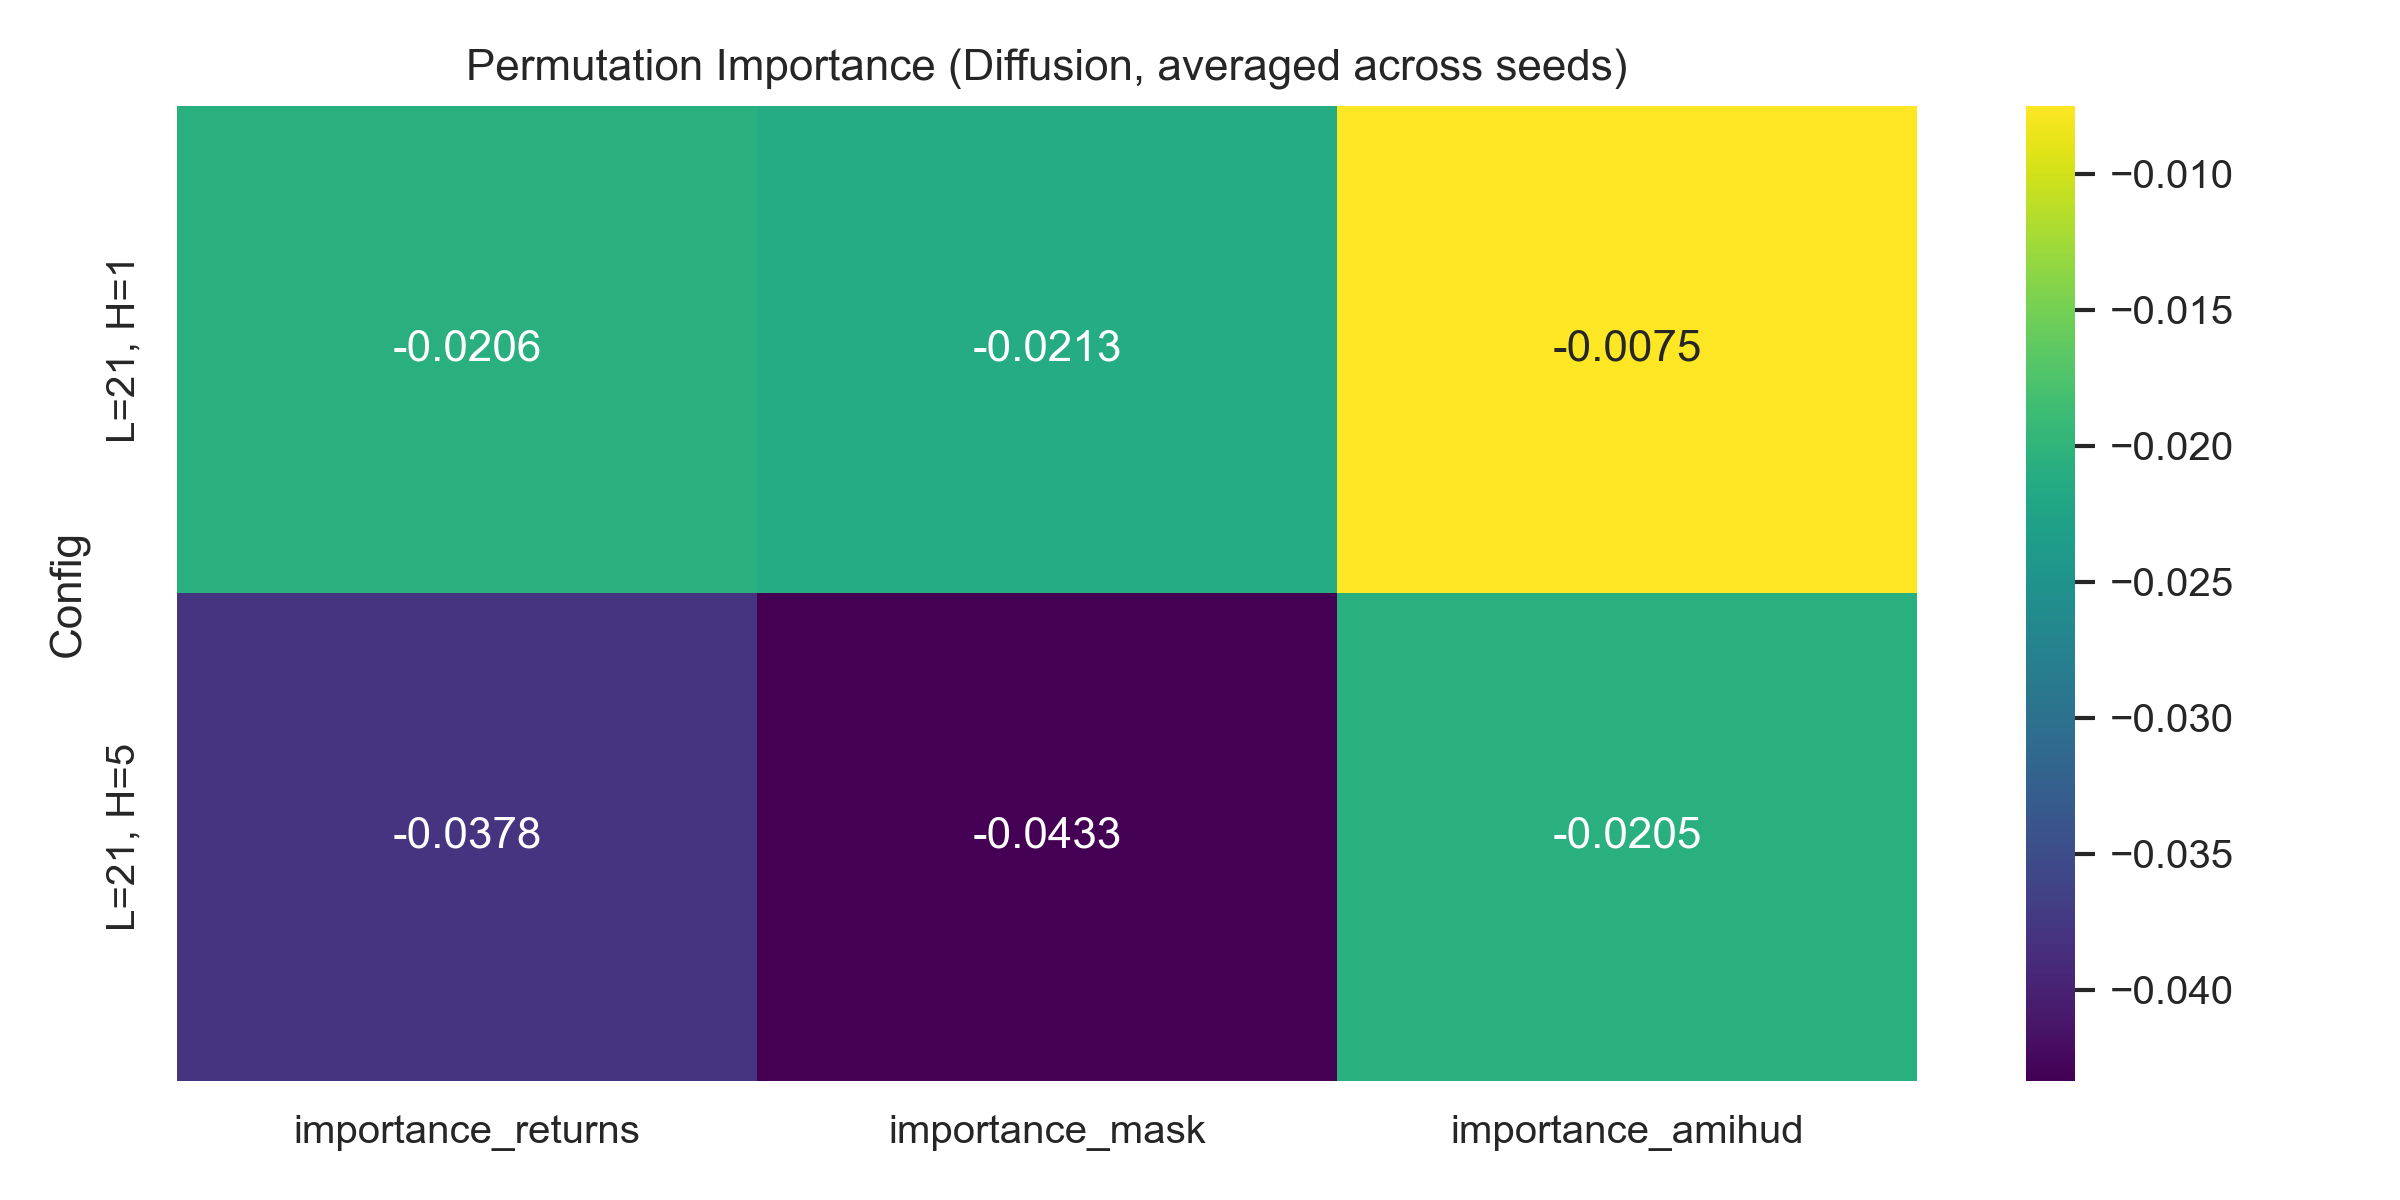
\includegraphics[width=\linewidth]{../figures/generated/fig_xai_importance_heatmap.png}
    \caption{Average permutation importance}
  \end{subfigure}
  \hfill
  \begin{subfigure}{0.49\linewidth}
    \centering
    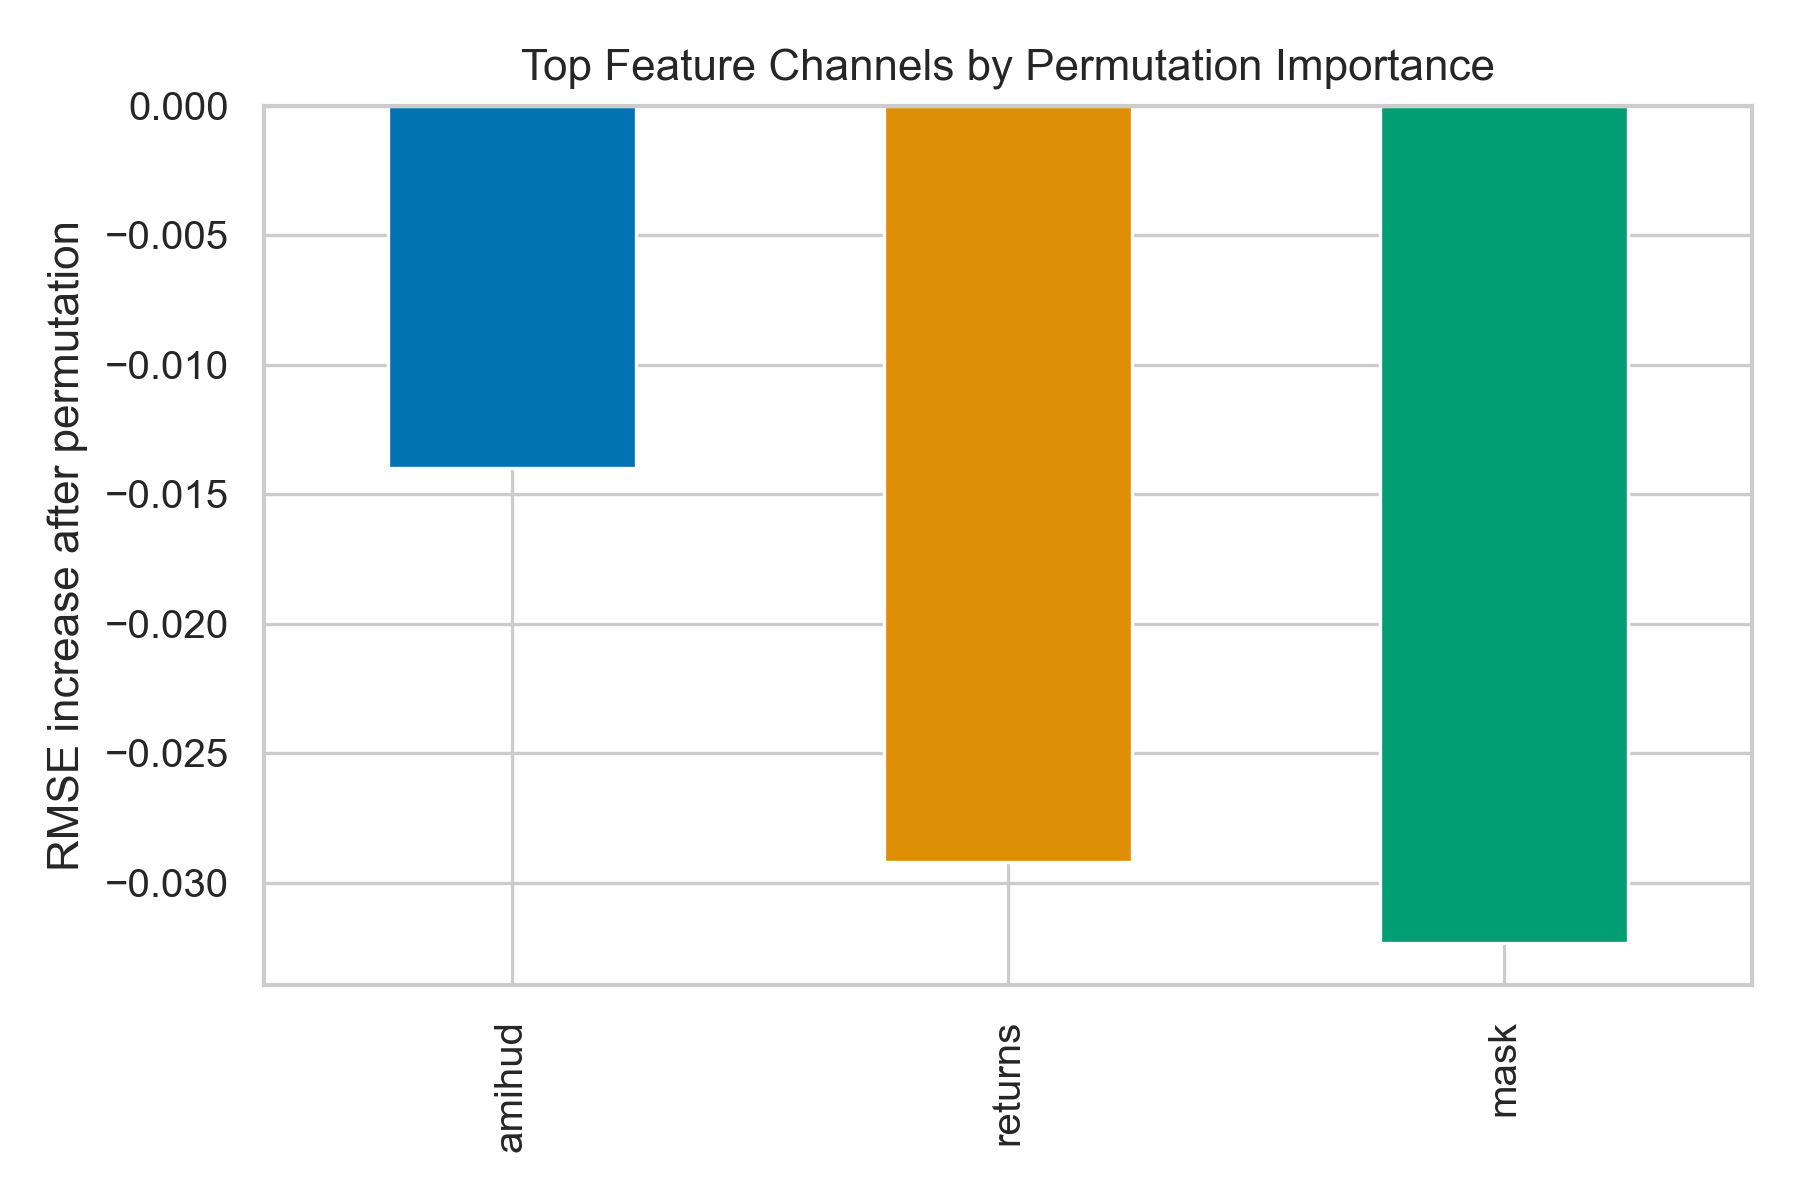
\includegraphics[width=\linewidth]{../figures/generated/fig_xai_top_features.png}
    \caption{Top feature channels}
  \end{subfigure}
  \caption{Diffusion model-reliance diagnostics from seed-level permutation analysis.}
  \label{fig:xai}
\end{figure}

\begin{table}[!htbp]
\centering
\caption{Permutation-importance max z-score sensitivity across diffusion seeds.}
\label{tab:xai-seed-sensitivity}
\begin{tabular}{lrrrr}
\toprule
L & H & Seed & Max z-score & Above 2.5 threshold \\
\midrule
21 & 1 & 0 & 1.170 & No \\
21 & 1 & 1 & 0.898 & No \\
21 & 1 & 2 & 1.189 & No \\
21 & 5 & 0 & 1.413 & No \\
21 & 5 & 1 & 1.414 & No \\
21 & 5 & 2 & 1.408 & No \\
\bottomrule
\end{tabular}
\end{table}

\begin{table}[!htbp]
\centering
\caption{XAI stability across seed pairs (Spearman correlation).}
\label{tab:xai-stability}
\begin{tabular}{lrrr}
\toprule
L & H & Seed pair & Spearman rho \\
\midrule
21 & 1 & 0-1 & 0.200 \\
21 & 1 & 0-2 & 0.400 \\
21 & 1 & 1-2 & -0.800 \\
21 & 5 & 0-1 & 0.400 \\
21 & 5 & 0-2 & 0.200 \\
21 & 5 & 1-2 & 0.800 \\
\bottomrule
\end{tabular}
\end{table}


XAI outputs are interpreted as model reliance only. \Cref{tab:xai-seed-sensitivity} shows no seed with max-\(z\) above 2.5, and \Cref{tab:xai-stability} shows unstable rank correlation across some seed pairs. Therefore, explanations are treated as fragile and non-structural.

\subsection{Robustness Checks and Sensitivity}
\begin{table}[!htbp]
\centering
\caption{Evaluation and leakage-control summary.}
\label{tab:robustness-summary}
\begin{tabular}{lr}
\toprule
Item & Value \\
\midrule
Evaluation windows & 5 \\
Total model-window evaluations & 330 \\
Leakage checks passed & True \\
Distinct benchmark models & 10 \\
MCS config rows & 6 \\
\bottomrule
\end{tabular}
\end{table}

\begin{table}[!htbp]
\centering
\caption{Diffusion sensitivity to feature-set ablations across seeds.}
\label{tab:diffusion-ablation}
\begin{tabular}{lrrrrr}
\toprule
L & H & Feature set & RMSE & MAE & RMSE std. \\
\midrule
21 & 1 & returns\_only & 0.02351 & 0.01599 & 0.00011 \\
21 & 1 & no\_illiquidity & 0.02352 & 0.01598 & 0.00010 \\
21 & 1 & full & 0.02375 & 0.01623 & 0.00023 \\
21 & 5 & full & 0.05334 & 0.03744 & 0.00005 \\
21 & 5 & returns\_only & 0.05344 & 0.03710 & 0.00008 \\
21 & 5 & no\_illiquidity & 0.05405 & 0.03759 & 0.00071 \\
\bottomrule
\end{tabular}
\end{table}

\begin{table}[!htbp]
\centering
\caption{Diffusion seed-level sensitivity by horizon and feature set.}
\label{tab:diffusion-seed-sensitivity}
\begin{tabular}{lrrrrr}
\toprule
L & H & Feature set & Seed & RMSE & MAE \\
\midrule
21 & 1 & full & 0 & 0.02375 & 0.01625 \\
21 & 1 & full & 1 & 0.02352 & 0.01599 \\
21 & 1 & full & 2 & 0.02398 & 0.01645 \\
21 & 1 & no\_illiquidity & 0 & 0.02360 & 0.01605 \\
21 & 1 & no\_illiquidity & 1 & 0.02356 & 0.01605 \\
21 & 1 & no\_illiquidity & 2 & 0.02341 & 0.01584 \\
21 & 1 & returns\_only & 0 & 0.02343 & 0.01592 \\
21 & 1 & returns\_only & 1 & 0.02364 & 0.01603 \\
21 & 1 & returns\_only & 2 & 0.02347 & 0.01603 \\
21 & 5 & full & 0 & 0.05340 & 0.03766 \\
21 & 5 & full & 1 & 0.05329 & 0.03732 \\
21 & 5 & full & 2 & 0.05334 & 0.03733 \\
21 & 5 & no\_illiquidity & 0 & 0.05355 & 0.03719 \\
21 & 5 & no\_illiquidity & 1 & 0.05374 & 0.03732 \\
21 & 5 & no\_illiquidity & 2 & 0.05487 & 0.03826 \\
21 & 5 & returns\_only & 0 & 0.05339 & 0.03702 \\
21 & 5 & returns\_only & 1 & 0.05353 & 0.03719 \\
21 & 5 & returns\_only & 2 & 0.05340 & 0.03710 \\
\bottomrule
\end{tabular}
\end{table}


\begin{figure}[!htbp]
  \centering
  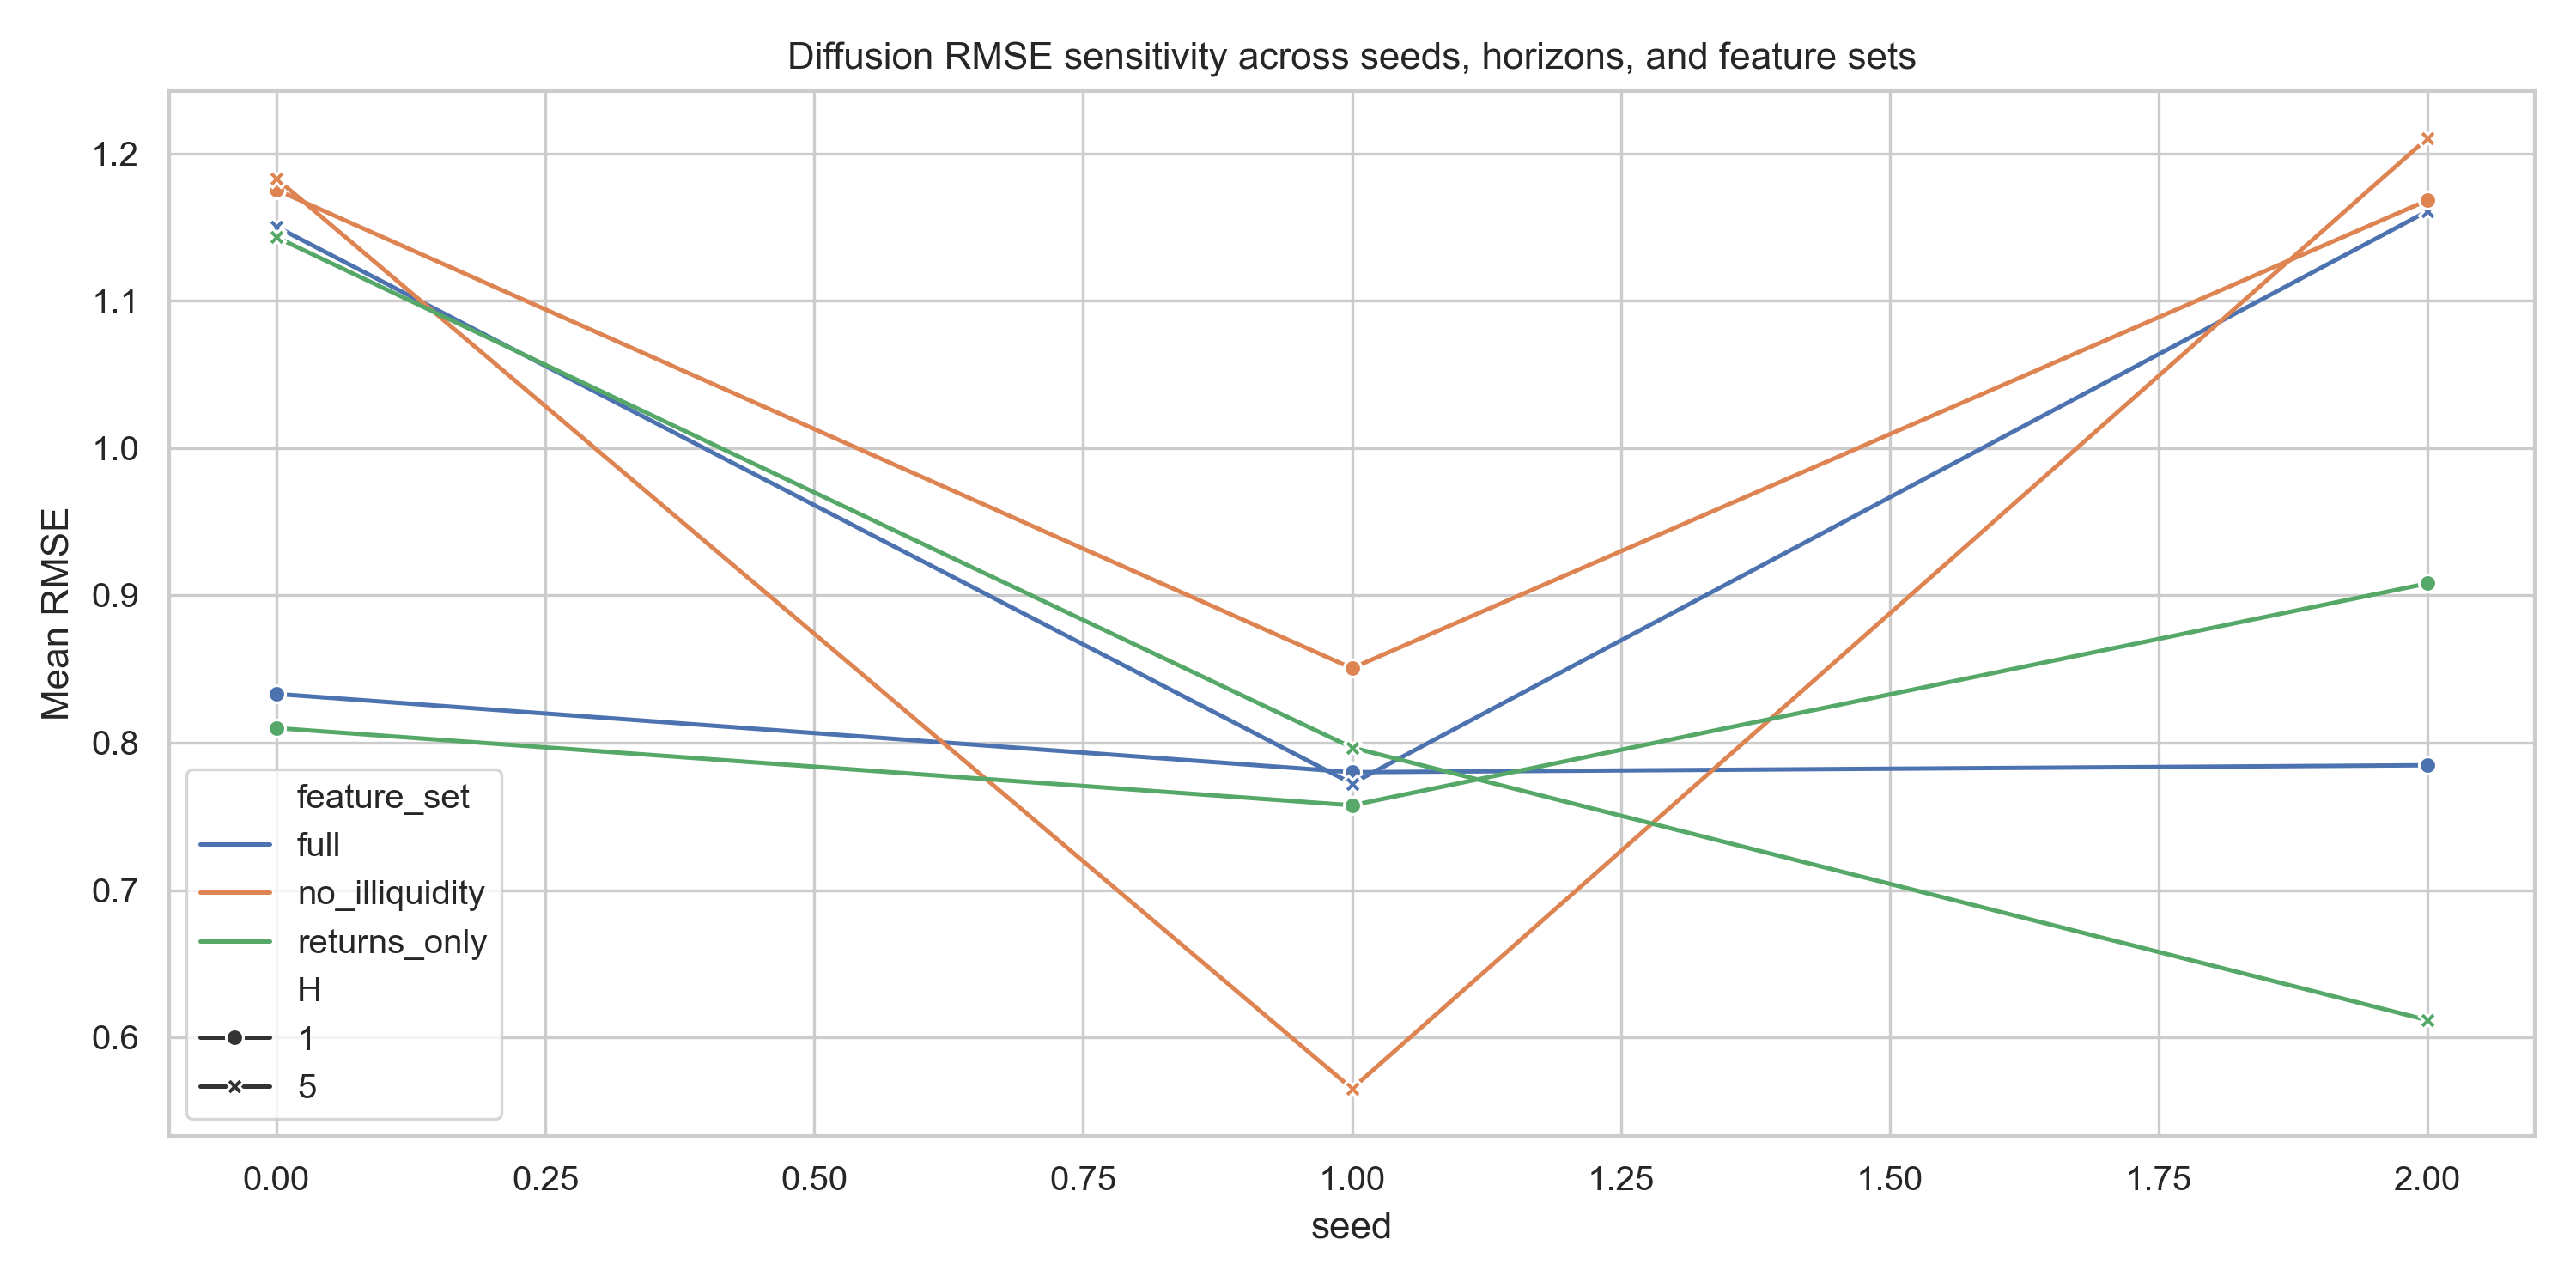
\includegraphics[width=0.84\linewidth]{../figures/generated/fig_diffusion_seed_sensitivity.png}
  \caption{Diffusion sensitivity across seeds, horizons, and feature sets.}
  \label{fig:diffusion-seed}
\end{figure}

Leakage assertions pass for all evaluation windows (\Cref{tab:robustness-summary}). Diffusion ablations in \Cref{tab:diffusion-ablation,tab:diffusion-seed-sensitivity,fig:diffusion-seed} indicate meaningful sensitivity to feature design and seed choice, with no robust improvement over benchmark models.

\subsection{EMH Interpretation}
Under a benchmark-relative predictability interpretation of weak-form EMH, the present evidence is consistent with limited extractable out-of-sample predictive gains beyond simple benchmarks in this dataset and design. This is a predictive, not structural, statement: the analysis does not establish exploitable abnormal profits, causal inefficiency mechanisms, or post-cost economic significance.

\section{Limitations and Remaining Robustness Boundaries}

The revised pipeline materially improves temporal integrity, benchmark breadth, and window-level evaluation; however, several boundaries remain.
\begin{enumerate}
  \item \textbf{Economic significance is not tested}: no transaction-cost-adjusted trading strategy is implemented, so forecast comparisons should not be interpreted as profitability evidence.
  \item \textbf{Model class coverage remains incomplete}: ARIMA/ARIMAX, GARCH-family, and VAR/VECM benchmarks are not yet included in the production loop.
  \item \textbf{Hyperparameter search is conservative}: diffusion and MLP settings use leakage-safe but limited tuning; nested time-series hyperparameter selection is not yet implemented.
  \item \textbf{Distributional validation is limited}: the current analysis emphasizes point-loss metrics; calibration-focused scoring and distributional diagnostics remain future work.
  \item \textbf{Inference depth}: DM comparisons are reported, but Model Confidence Set procedures \parencite{hansen2011} are not yet integrated.
  \item \textbf{Data scope}: conclusions are specific to four ETF proxies and the 2015--2023 sample, and may not generalize to other assets, frequencies, or post-2023 regimes.
\end{enumerate}

\section{Conclusion}

This paper evaluates weak-form EMH through benchmark-relative forecast testing, not structural market-efficiency identification. Under expanding-window evaluation, leakage controls, multiple loss metrics, and a stronger benchmark family, random walk remains the best-performing model by RMSE across all tested \((L,H)\) settings.

Conditional diffusion does not provide incremental predictive gains in this implementation and is significantly worse than random walk in all Diebold--Mariano comparisons. Diffusion ablation and seed analyses also indicate sensitivity rather than stable superiority. XAI outputs, interpreted as model reliance diagnostics, are not stable enough to support strong economic narratives.

The main contribution is therefore methodological: a transparent, reproducible, benchmark-disciplined pipeline for weak-form predictability testing in Latin American ETF proxies, including explicit robustness boundaries and interpretation discipline. Stronger claims would require broader benchmark classes, deeper hyperparameter validation, and an explicit post-cost economic significance layer.


\appendix
\section{Supplementary Diagnostics and Reproducibility Notes}

The robust experiment loop writes diagnostics and evaluation outputs to \path{reports/tables/}, including:
\begin{enumerate}
  \item \path{per_window_losses.csv} (window-level RMSE, MAE, directional accuracy);
  \item \path{leakage_checks.csv} (horizon-overlap assertions);
  \item \path{diffusion_training_stability.csv} (best-epoch and validation-loss summaries);
  \item \path{diffusion_seed_sensitivity.csv} and \path{diffusion_ablation.csv};
  \item \path{xai_seed_sensitivity.csv} and \path{xai_stability.csv}.
\end{enumerate}

Manuscript asset generation is scripted via \path{scripts/build_manuscript_assets.py}, which converts report CSV files into \path{tables/generated/*.tex} and copies standardized figures to \path{figures/generated/}. Overleaf package export is automated by \path{scripts/build_working_paper.py}.


\bibliographystyle{apalike}
\bibliography{../paper/references}

\end{document}
